\documentclass[10pt,conference]{IEEEtran}

\usepackage[utf8]{inputenc}
\usepackage[ngerman]{babel}
\usepackage{graphicx}

\begin{document}
	
\title{Advanced Programming Concepts for Software-defined Networks (SDN)}
\author{
	\IEEEauthorblockN{Stefan Schmid}
	\IEEEauthorblockA{Universität Stuttgart\\
		Universitätsstraße 38\\
		D-70569 Stuttgart\\
		Matrikelnummer: 3102206\\
		Email: st140748@stud.uni-stuttgart.de\\ \\
		Betreuer: Ruben Mayer, Institut für Parallele und Verteilte Systeme (IPVS)}
}
\date{\today}
\maketitle

\begin{abstract}
Diese Ausarbeitung befasst sich mit dem Vergleich zweier High-Level-Programmiersprachen für Software-defined Networks (SDN).\\
Die Ansätze von Frenetic \cite{2,3,4,6} und Maple \cite{7,10} versprechen durch das hohe Abstraktionslevel eine deutlich einfachere Programmierung für die Entwickler. Dabei verfolgen die zwei genannten Sprachen jedoch verschiedene Grundideen, die ich im folgenden genauer beleuchten möchte. 
\end{abstract}

\section{Einleitung}
Die Anforderungen an Netzwerke haben sich in den letzten Jahren stark verändert.\\
Vor allem Cloud-Anwendungen und Virtualisierung erfordern ein hohes Maß an Flexibilität innerhalb der Netzwerkstruktur, um z.B. optimale Lastverteilung zu garantieren.\\
Ein verbreiteter Ansatz, um sich diesen Herausforderungen anzunehmen, stellen die Software-defined Networks dar.\\ 
Der Trend geht dabei weg von statischen Netzwerken hin zu dynamischeren um automatisiert auf geänderte Anforderungen reagieren zu können. \cite{1}[S. 36]

\section{Software-defined Networks (SDN)}
\begin{figure}[h]
	\centering
	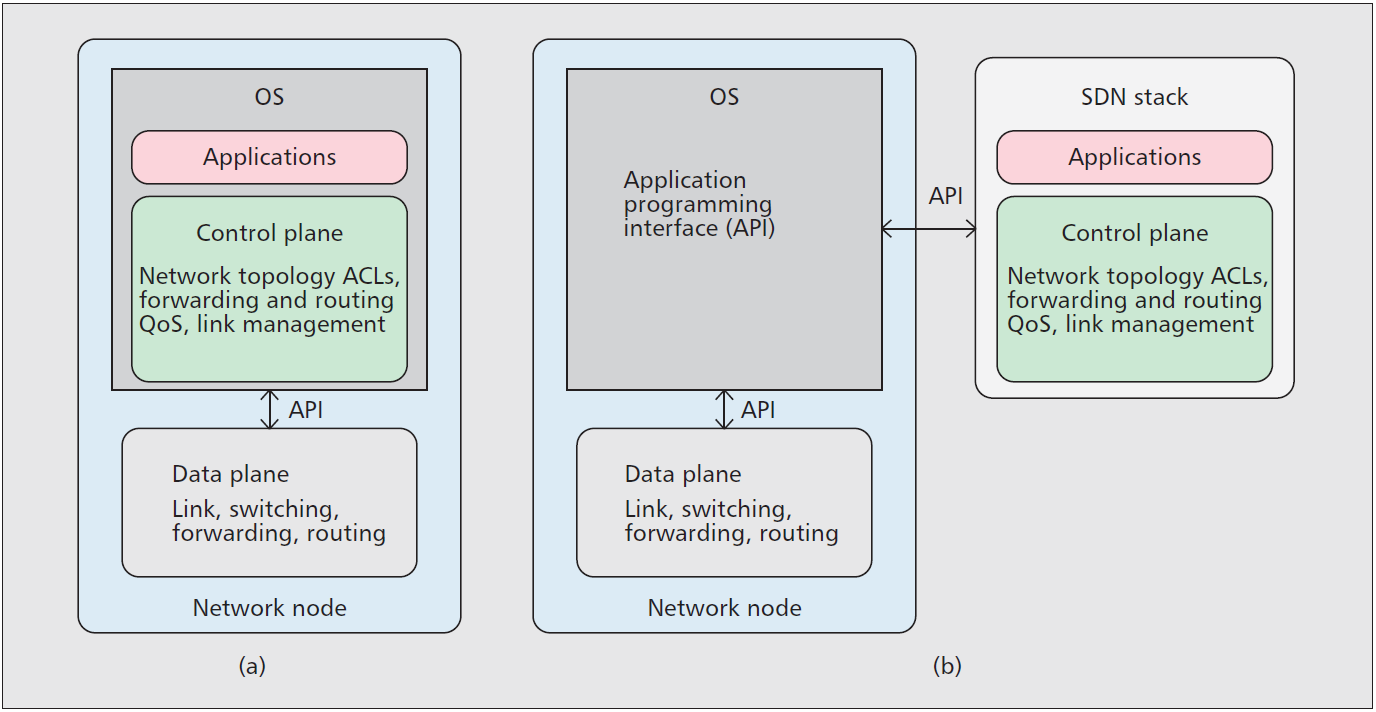
\includegraphics[width=\columnwidth]{images/VergleichHerkoemmlichSDN.PNG}
	\caption{Vergleich der herkömmlichen mit der SDN-Netzwerksicht. a) Herkömmlicher Ansatz b) SDN-Ansatz \cite{1}[S. 38]}
	\label{fig:VergleichHerkoemmlichSDN}
\end{figure}
Software Defined Networks (SDN) verfolgen den Ansatz, die Kontrollschicht von der Datenschicht zu abstrahieren.\\
In Abbildung \ref{fig:VergleichHerkoemmlichSDN} ist auf der linken Seite schön der traditionelle Ansatz der Netzwerksicht zu sehen. Jeder Knoten beherbergt dabei sein eigenes Betriebssystem, auf welchem Anwendungen und die Routing-Logik läuft. Über eine interne API steuert dieses Betriebssystem die darunterliegende Datenschicht an, welche z.B. für Switching und Forwarding relevant ist. \cite{1}[S. 37], \cite{5}, \cite{11} \\
\newline
Im Gegensatz wird bei SDNs die Kontrollschicht von den einzelnen Knoten ausgelagert und zentralisiert. Über eine API können auch hier die Knoten angesprochen werden, welche nur noch die untere Datenschicht enhalten, also die Abwicklung zur physischen Übertragung. \cite{1}[S. 38] 
\begin{figure}[h]
	\centering
	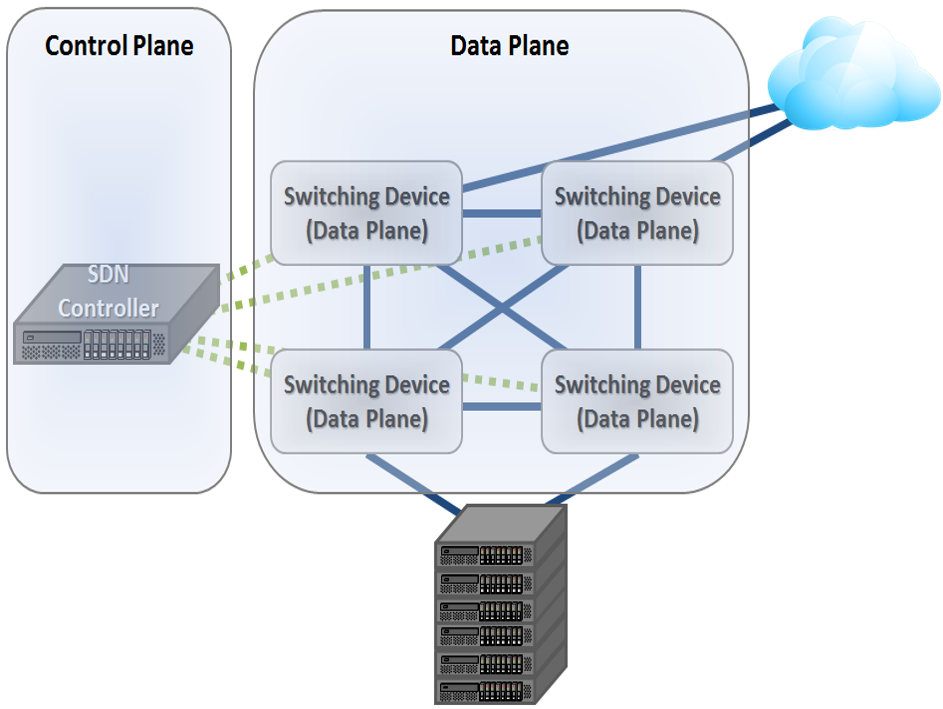
\includegraphics[width=\columnwidth]{images/control-data-plane.png}
	\caption{Trennung von Kontroll- und Datenschicht in SDN-Netzwerken \newline http://www.definethecloud.net/wp-content/uploads/2012/06/image1.png \newline (aufgerufen am 04.02.2016)}
	\label{fig:SDN_controlDataPlane}
\end{figure}

\section{OpenFlow Protokoll}
OpenFlow ist ein öffentliches Protokoll, um in  OpenFlow-fähigen Switches und Routern die Einträge der flow-tables zu manipulieren. \cite{9}[S. 70] \\
In Abbildung \ref{fig:openflowSwitch} wird die grundlegende Spezifikation eines OpenFlow Switches schön dargestellt. Dabei besteht ein OpenFlow Switch aus einem Hardware- als auch einem Software-Teil. Die obere Softwareebene überlagert die Hardware und kommuniziert über das OpenFlow Protokoll mit dem Controller (z.B. NOX \cite{8}), welcher das SDN verwaltet.\\
Innerhalb der Switches/Router liegt die sogenannte Flow Table auf der Hardwareebene. Sie enthält Forwarding-Regeln für Pakete, deren Header auf bestimmte Patterns matchen und kann über die Softwareschicht von extern über einen Controller manipuliert werden. \cite{9}[S. 70-71], \cite{11}
\begin{figure}[h]
	\centering
	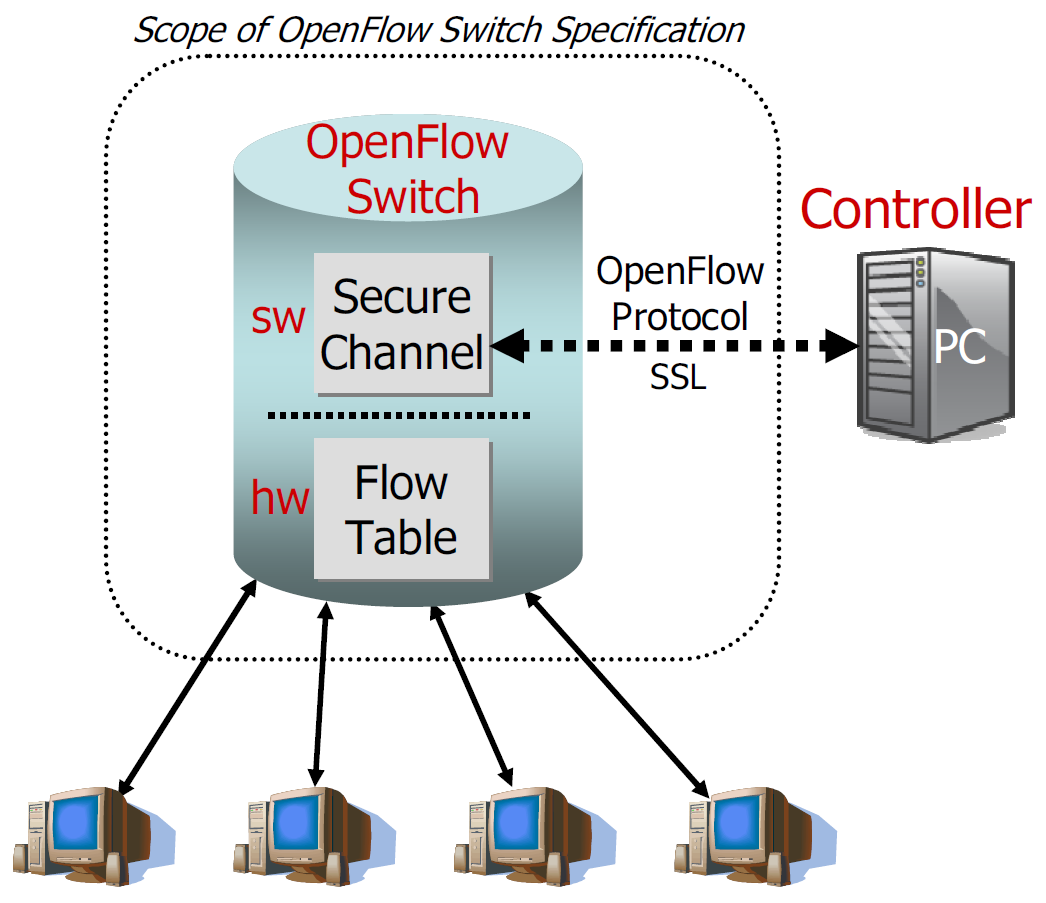
\includegraphics[width=\columnwidth]{images/openflowSwitch.PNG}
	\caption{Grundlegende Spezifikation eines OpenFlow Switches \cite{9}[S. 70]}
	\label{fig:openflowSwitch}
\end{figure}
\newline
Die Einträge der Flow Table unterliegen der formalen Definition aus Abbildung \ref{fig:openflowDefinition}. 
\begin{figure}[h]
	\centering
	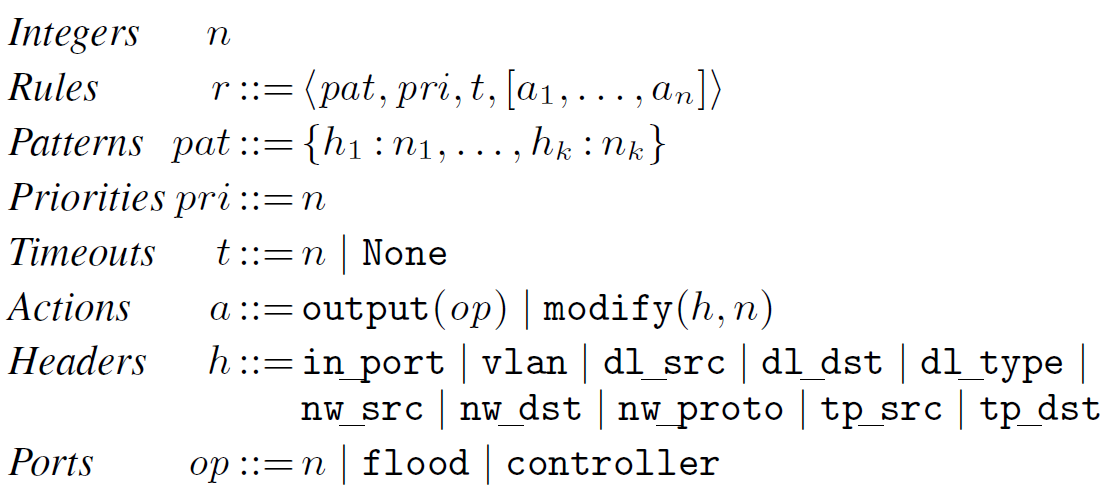
\includegraphics[width=\columnwidth]{images/openflowDefinition.PNG}
	\caption{Definiton der OpenFlow-Grammatik \cite{4}[S. 280]}
	\label{fig:openflowDefinition}
\end{figure}
\newline
Tatsächlich in der Tabelle werden dabei die Regeln (Rules) gespeichert. Diese bestehen aus Patterns, welche auf die Paketheader gematched werden, einer Priorität, einem optionalen Timeout und mehreren Aktionen, die für passende Pakete auf das bereits definierte Pattern durchgeführt werden sollen.\\
Ein Pattern besteht aus mehreren möglichen Header-Informationen, wie z.B. der Quell- oder Ziel-IP-Adresse des Pakets, dem Eingangsport etc.\\
Die Priorität einer Regel wird über einen simplen Integer-Wert festgelegt, genauso wie auch der Timeout der Regel.\\
Die durchzuführende Aktion einer Regel kann entweder eine Weiterleitung oder Modifikation des Paket-Headers sein. \\
Üblicherweise führen OpenFlow Switches auch noch einen Zähler je installierter Regel mit für eventuelle Statistikverwendung. \cite{4}[280], \cite{11}\\
\newline
Die Abarbeitung eines Pakets im OpenFLow Switch läuft im Allgemeinen in 3 Stufen ab: \cite{4}[S. 280] \cite{1}
\begin{enumerate}
	\item Anwendung deiner passenden Regel aus der Flow Table. Im Fall, dass diese nicht existiert, wird das Paket direkt an den Controller weitergeleitet und dort weiter verarbeitet.
	\item Inkrementierung der Zähler für die entsprechenden Regeln
	\item Anwendung der ermittelten Aktionen auf das erhaltene Paket
\end{enumerate}

\section{NOX Controller}
Einer der bekanntesten, mehrfach schon erwähnten SDN-Controller ist NOX \cite{8}. Er repräsentiert die Control Plane, wie in Abbildung \ref{fig:SDN_controlDataPlane} bereits erwähnt.\\
NOX versteht sich als eine Art Betriebssystem für Netzwerke. Es abstrahiert die Netzwerksicht auf einem niedrigen Level, sodass nicht mehr mit Maschinencode Vorlieb genommen werden muss.\\
Darauf aufbauend können Anwendungen für die Netzwerke geschrieben werden. \cite{8}[S. 105]\\
Ein NOX Controller arbeitet eventgesteuert, d.h. es gibt einen Satz an Funktionen, die auf ein bestimmtes Netzwerkverhalten ausgeführt werden: \cite{4},[S. 281] \cite{8}[S. 107-108]
\begin{itemize}
	\item \textbf{packet\_in(switch,port,packet)}\\
	Wird getriggert, wenn ein OpenFlow Switch ein Paket an den Controller weiterleitet.
	\item \textbf{stats\_in(switch,xid,pattern,packets,bytes)}\\
	Wird getriggert, sobald der OpenFLow Switch die angeforderten Paket- und Byte-Zähler an den Controller zurück liefert.
	\item \textbf{flow\_removed(switch,pattern,packets,bytes)}\\
	Wird getriggert, wenn eine Regel aufgrund ihres Timeouts entfernt wurde. Die finalen Paket- und Byte-Zähler werden automatisch mit geliefert.
	\item \textbf{switch\_join(switch)}\\
	Wird getriggert, sobald ein neuer Switch dem Netzwerk beitritt.
	\item \textbf{switch\_exit(switch)}\\
	Wird getriggert, sobald ein Switch das Netzwerk verlässt.
	\item \textbf{port\_change(switch,port,up)}\\
	Wird getriggert, sobald an einem Switch ein Port geöffnet oder geschlossen wird.
\end{itemize}
Um auf die eben genannten Events reagieren zu können, können die OpenFlow Switches über folgende vordefinierte Funktionen manipuliert werden: \cite{4},[S. 281] \cite{8}[S. 107-108]
\begin{itemize}
	\item \textbf{install(switch,pattern,priority,timeout,actions)}\\
	Installiert eine neue Regel in der Flow Table
	\item \textbf{uninstall(switch,pattern)}\\
	Entfernt eine bestehende Regel aus der Flow Table
	\item \textbf{send(switch,packet,action)}
	Sendet ein Paket an einen Switch mit einer bestimmten Anweisung zur Weiterleitung.
	\item \textbf{query\_stats(switch,pattern)}\\
	Löst eine Anfrage der Paket- und Byte-Zähler aller Regeln mit einem bestimmten Pattern aus.
\end{itemize}

\section{Probleme bei der NOX-Programmierung von OpenFlow-Netzwerken}
Generell erscheint der überschaubare Satz an Events und Send-Methoden eines NOX-Controllers aus dem vorigen Kapitel einleuchtend und relativ simpel in der Implementierung.\\
Das Beispiel eines einfachen Repeaters mit Python und NOX aus Abbildung \ref{fig:NOXRepeaterPrimitive} bestätigt diese These auch zunächst. Eine Repeater-Methode installiert dabei zwei Regeln im Switch. Eine soll von Port 2 auf Port 1 weiterleiten und die andere genau umgekehrt von Port 1 auf Port 2.\\
Über das in NOX definierte switch\_join-Event werden für jeden neu hinzugefügten Switch die repeater-Methode aufgerufen und damit die zwei Regeln in der Flow Table installiert. \cite{4}[S. 281]\\
Dieses einfache Programm stellt durch die Implementierung des passenden Events bereits sicher, das sich das SDN-Netzwerk physisch ändern darf. Dabei spielt es auch keine Rolle mehr, von welchem Hersteller die Switches stammen, denn nur die standardisierte OpenFlow-Schnittstelle muss angesprochen werden.
\begin{figure}[h]
	\centering
	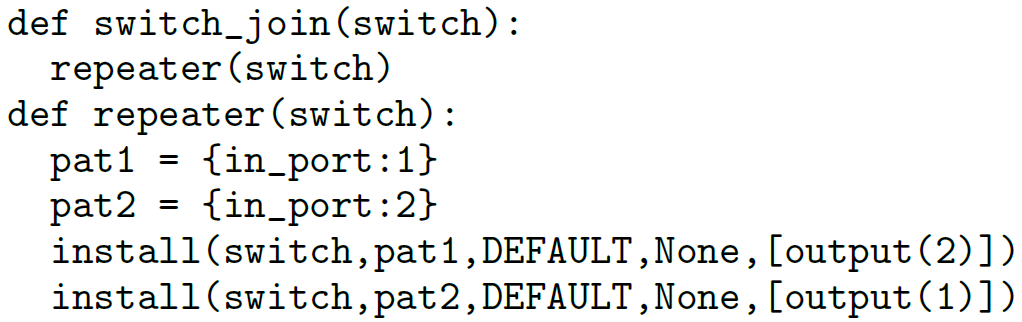
\includegraphics[width=\columnwidth]{images/NOXRepeaterPrimitive.PNG}
	\caption{Einfacher Repeater in Python, aufbauend auf NOX \cite{4}[S. 281]}
	\label{fig:NOXRepeaterPrimitive}
\end{figure}
\newline
Möchte man nun den Repeater aus Abbildung \ref{fig:NOXRepeaterPrimitive} um ein Monitoring erweitern, offenbaren sich schnell versteckte Fehlerursachen, auch wenn die Programmlogik korrekt zu sein scheint.\\
Wir möchten nun die grundlegende Repeater-Funktionalität um ein Logging der Paketzahlen, welche ausgehend von HTTP-Port 80 an Port 2 eines Switches eintreffen.\\
Dafür werden in Abbildung \ref{fig:NOXRepeaterMonitoringFunctions} ganz primitiv zwei Methoden implementiert, eine zur Installation des gewünschten Monitoring-Patterns, als auch die Event-Funktion, welche die Daten erhalten soll.\\
Die monitor-Funktion installiert die Regel mit Quellport 80 und Eingangsport 2 im Switch. Danach wird direkt über die NOX-Funktion query\-stats die Anforderung der Zählerstände angefordert.\\
In der zugehörigen Event-Methode stats\_in werden die Anzahl der bisherigen Bytes ausgegeben und nach 30 Sekunden rekursiv eine neue Anfrage gestartet. Dies hat zur Folge, dass der Zählerstand alle 30 Sekunden ausgegeben wird. \cite{4}[S. 281]
\begin{figure}[h]
	\centering
	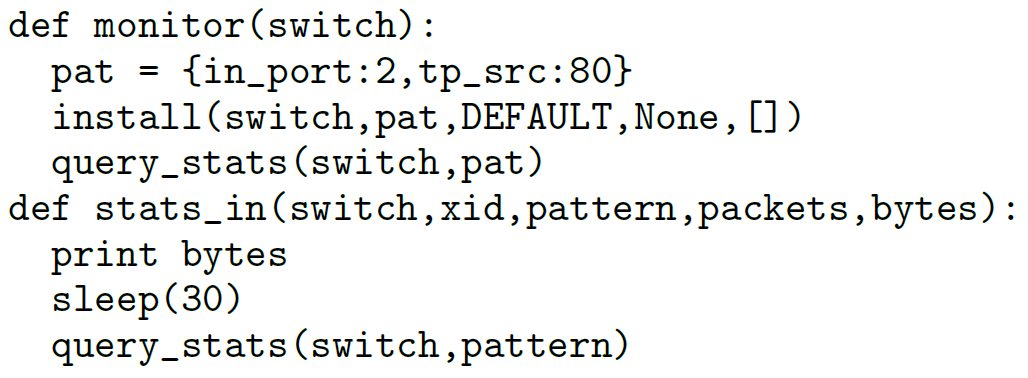
\includegraphics[width=\columnwidth]{images/NOXRepeaterMonitoringFunctions.PNG}
	\caption{Erweiternde Methoden, für das Monitoring des Repeaters \cite{4}[S. 281]}
	\label{fig:NOXRepeaterMonitoringFunctions}
\end{figure}
\newline
Abschließend muss noch die Repeater- und Monitoring-Funktionalität verschmolzen werden. Intuitiv ruft man dazu wie in Abbildung \ref{fig:NOXRepeaterMonitoringWrong} die Repeater und die Monitoring-Funktion nacheinander auf, um die entsprechenden Regeln zu installieren.
\begin{figure}[h]
	\centering
	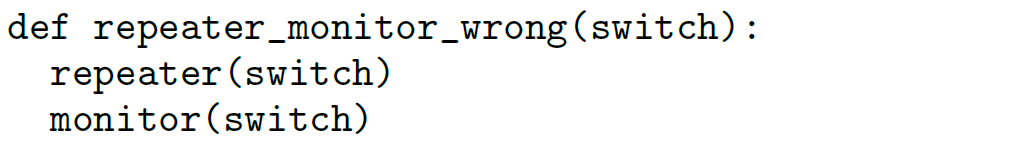
\includegraphics[width=\columnwidth]{images/NOXRepeaterMonitoringWrong.PNG}
	\caption{Vermeintliche Verschmelzung des Repeaters mit der neuen Monitoring-Funktionalität \cite{4}[S. 281]}
	\label{fig:NOXRepeaterMonitoringWrong}
\end{figure}
\newline
Das Problem mit dieser Implementierung stellen die resultierenden, überlappenden Regeln der Flow Table dar.\\
Sobald ein Paket an Port 2 ankommt, wird genau eine passende Regel aus der Flow Table gewählt, d.h. es kann nie gesagt werden, ob ein Paket, welches von Port 80 an Port 2 eintrifft gezählt wird oder nicht.\\
Genau dieses Problem mit überlappenden Regeln ist der Grund dafür, weshalb es keine allgemeingültigen Libraries für bestimmte Monitoring-Funktionalitäten geben kann. \cite{4}[S. 182]\\
Der Repeater-Monitor kann jedoch mittels Prioritäten (siehe Abbildung \ref{fig:NOXRepeaterMonitoring}) in den installierten Regeln so umgesetzt werden, dass alle Pakete ausgehend von Port 80 und ankommend an Port 2 sowohl weitergeleitet als auch gezählt werden.
\begin{figure}[h]
	\centering
	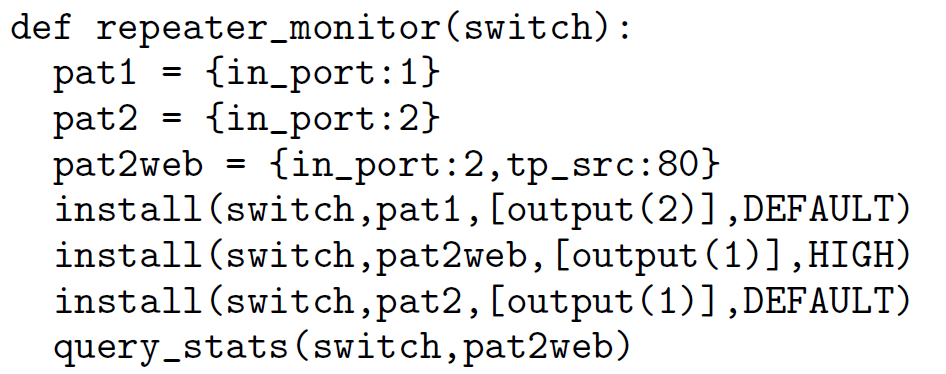
\includegraphics[width=\columnwidth]{images/NOXRepeaterMonitoring.PNG}
	\caption{Korrekte Verschmelzung des Repeaters mit der neuen Monitoring-Funktionalität \cite{4}[S. 281]}
	\label{fig:NOXRepeaterMonitoring}
\end{figure}
\newline
Unabhängig von den Problemen mit überlappenden Regeln, macht das Low-Level Interface Ärger. Eine einfache logische Differenz zwischen zwei Patterns muss mit überlappenden Regeln und unterschiedlichen Prioritäten gesteuert werden. Dadurch wird zum einen die Komplexität für den Programmierer enorm gesteigert, als auch die spätere Nachvollziehbarkeit des Codes erheblich erschwert.\\
Weitere Schwierigkeiten bereiten z.B. asynchrone, parallele Anwendungen, bei denen Pakete nicht in einer festgelegten Reihenfolge eintreffen müssen.\\
Dies kann zu Race Conditions führen, wenn abhängig vom ersten Paket eines Datenstroms eine Regel zur Abarbeitung der nachfolgenden Pakete erfolgen soll. Trifft z.B. das zweite Datenpaket vor dem ersten ein und der Controller kann dieses nicht handeln, da es nicht das erste Paket des Datenstroms ist, so schlägt das Routing bereits hier fehl. \cite{4}[S. 282]

\section{Frenetic}
Frenetic versucht sich nun durch ein höheres Abstraktionslevel, aufbauend auf NOX, den eben aufgezeigten Problemen anzunehmen. \cite{4}\\
Ein hohes Abstraktionslevel verspricht meistens eine einfachere Implementierung von Anwendungen, doch wir möchten auch die technischen Hintergründe näher beleuchten.\\
Zu Beginn liegt der Fokus aber erst einmal auf den Möglichkeiten, die der deklarative und funktionale Ansatz bietet. Für den Programmierer stehen dazu die Network Query Language und die Network Policy Management Library bereit. \cite{3,4}

\subsection{Network Query Language}
Die Query Language von Frenetic (siehe Abbildung \ref{fig:freneticQuerySyntax}) erlaubt es dem Programmierer, den aktuellen Netzwerkzustand auszulesen.
\begin{figure}[h]
	\centering
	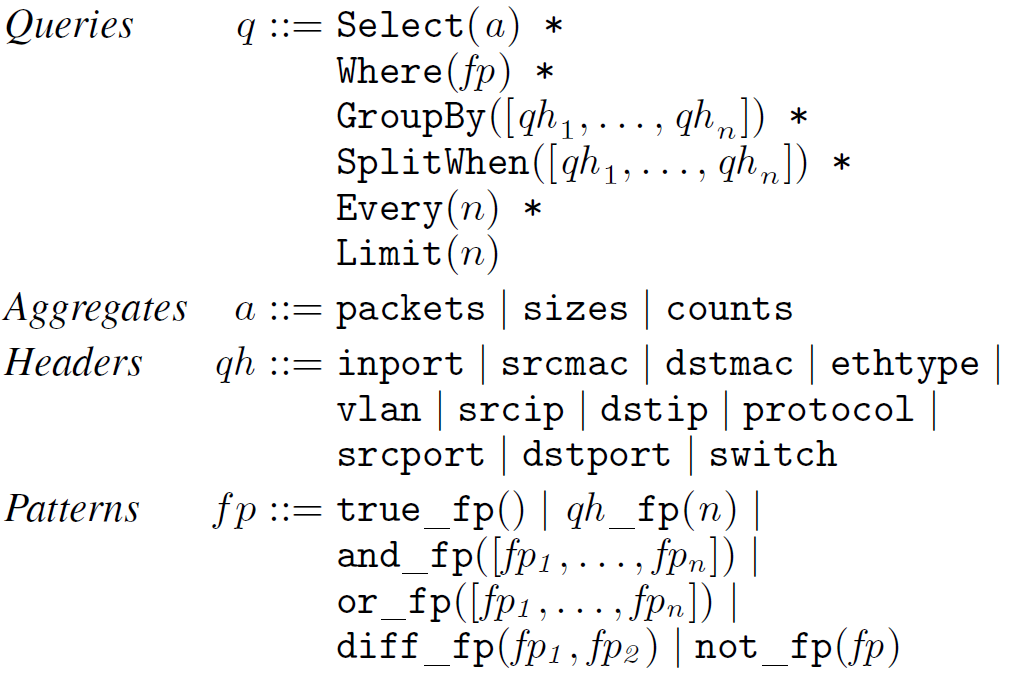
\includegraphics[width=\columnwidth]{images/freneticQuerySyntax.PNG}
	\caption{Grammatik der Frenetic Network Query Language \cite{4}[S. 283]}
	\label{fig:freneticQuerySyntax}
\end{figure}
\newline
Die SQL-ähnliche, deklarative Syntax erlaubt es, aggregierte Werte für Pakete, Paketgrößen als auch Paketzahlen für bestimmte Filter Patterns abzufragen. Diese werden auf die Paketheader gematcht, d.h. z.B. den Eingangsport, das verwendete Protokoll, die Ziel-IP-Adresse usw.\\ 
Eine boolsche Verknüpfung dieser Filter Patterns ist analog zu SQL ebenso möglich.\\
Über das GroupBy-Statement besteht die Möglichkeit, die gefilterten (aggregierten) Werte in kleinere Subsets mit beispielsweise gleicher Ziel-IP-Adresse zu unterteilen. Dies kann im Hauptprogramm die Analyse der Informationen deutlich vereinfachen. \cite{4}[S. 283]\\
Das SplitWhen-Statement ermöglicht ähnlich wie GroupBy eine Unterteilung in Subsets. Die Besonderheit besteht jedoch darin, dass nur aufeinanderfolgende, identische Werte in einem Set zusammengefasst werden. Für jeden Wechsel wird generell ein neues Set angelegt. \cite{4}[S. 283]\\
\textbf{Bsp.:} Folge von Ziel-IP-Adressen (dstip)
\begin{center}
	(1.1.1.1) (1.1.1.1) (2.2.2.2) (1.1.1.1)
\end{center}
Erzeugte Subsets für ...SplitWhen(dstip)...
\begin{enumerate}
	\item (1.1.1.1) (1.1.1.1)
	\item (2.2.2.2)
	\item (1.1.1.1)
\end{enumerate}
Durch Every können die Pakete schlussendlich noch in einem angegebenen Zeitintervall zusammengefasst werden und durch Limit die Anzahl der Pakete je Subset beschränkt werden. \cite{4}[S. 283]\\
\newline
Durch den deklarativen Ansatz beschreibt der Programmierer nur noch, welche Werte er auf welche Weise zusammengefasst haben möchte. Wie das darunterliegende System die Werte ermittelt, spielt dabei aus Entwickler-Sicht keine Rolle.\\ 
Dafür ist einzig und allein das Frenetic Run-Time System zuständig, welches im weiteren Verlauf genauer analysiert wird. \cite{3}[S. 5]

\subsection{Network Policy Management Library}
Die Network Policy Management Library (Auszug siehe Abbildung \ref{fig:freneticNetworkPolicyManagementLibrary}) ist eine sogenannte Combinator Library \cite{12}[S. 35-36].\\ 
Sie ist ein Teil funktionaler reaktiver Programmierung (FRP) \cite{u1} und verfolgt die Idee, durch Kombination bestehender Funktionen noch mächtigere Funktionen zu kreieren. \\
Funktionale reaktive Programmierung ist ein Paradigma, um eventgesteuerte Systeme deklarativ zu programmieren. \cite{12,u1}\\
Der reine NOX Controller ist (siehe vorherige Kapitel) bereits event-gesteuert, doch Frenetic abstrahiert diese Ebene grob gesagt noch durch funktionale Programmierung, um das Hauptproblem überlappender Regeln aus Anwendersicht zu beheben. \cite{3} \\
Der Grundgedanke der Architektur ist, dass das System jedes Paket zu jeder Zeit sieht, zumindest aus Programmierersicht. \cite{3}[S. 3]\\
\newline
Ein Auszug der Definitionen von Events und Listeners ist in Abbildung \ref{fig:freneticNetworkPolicyManagementLibrary} zu sehen.\\
\newline
\textit{Events} repräsentieren bestimmte eintreffende Zustände im Netzwerk, auf die im Programm reagiert werden kann. SwitchJoin trifft ein, sobald ein Switch dem Netzwerk beitritt und liefert den entsprechenden Switch zurück. Analog dazu existiert SwitchExit, sobald ein Switch aus dem Netzwerk ausscheidet.\\
Das PortChange-Event geht in dieser Hinsicht deutlich tiefer und reagiert auf jede Aktivierung, sowie Deaktivierung von Switch-Ports. Hier wird der Switch mit einem Boolean für die Aktivierung und der entsprechenden Port-Nummer zurück geliefert. \cite{4}[S. 285-286]\\
\newline
\textit{Basic Event Functions} überführen dagegen normale Funktionen in Eventfunktionen.\\
Dies bedeutet umgangssprachlich, dass die normale Funktion bei Lift z.B. auf alle Eingabeevents angewendet wird. Bei ApplyFst und ApplySnd würde dies nur für das erste, bzw. zweite Eingabeevent zutreffen. \cite{4}[S. 286]\\
Über die Filter-Funktion können Pakete nach bestimmten Patterns selektiert werden. \cite{3}[S. 3]
\begin{figure}[h]
	\centering
	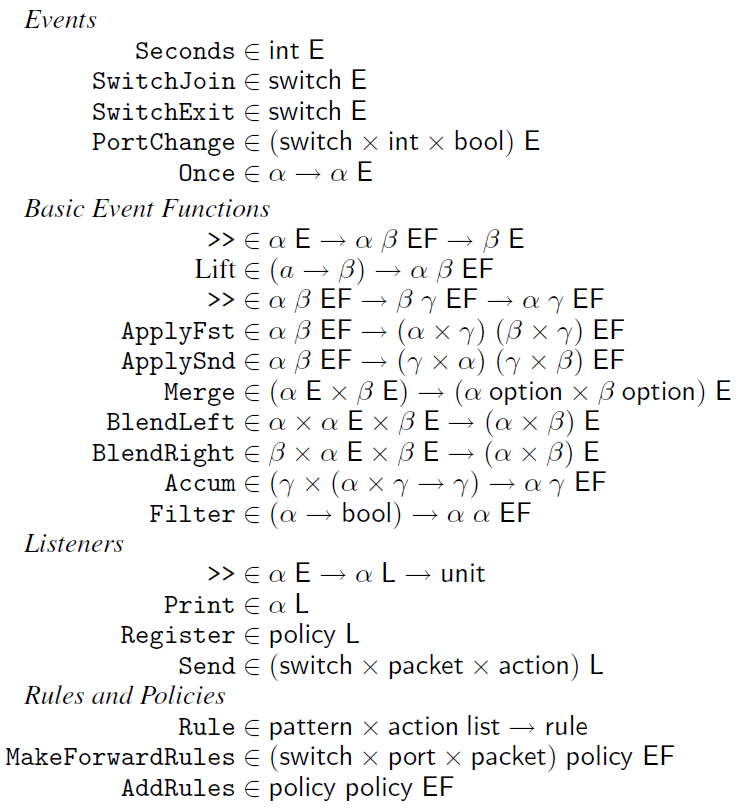
\includegraphics[width=\columnwidth]{images/freneticNetworkPolicyManagementLibrary.PNG}
	\caption{Auszug der Frenetic Network Policy Management Library\cite{4}[S. 283]}
	\label{fig:freneticNetworkPolicyManagementLibrary}
\end{figure}
\newline
\textit{Listeners} sind dafür zuständig, Aktionen auf dem Netzwerk oder Logging durchzuführen. Die Print-Funktion schreibt beispielsweise nur den Input auf die Konsole, während Register die übergebenen Strategien in den Switches installiert. Send erhält ein Event, durch welches ein bestimmtes Paket an einen bestimmten Switch gesandt und dort dann die mitgeführte Aktion getätigt wird. \cite{3}[S. 285-286]\\
\newline
\textit{Rules and Policies} stellen den letzten Unterpunkt dar. Über Rule können Regeln mit definierten Patterns und Aktionen erzeugt werden. Diese Regeln können auch automatisiert über MakeForwardRule erzeugt werden. Dabei wird eine Forwarding Regel für alle Pakete mit identischem Header zum übergebenen Paket erzeugt. Diese gilt für einen festgelegten Switch und dortigen Port.\\
AddRules merged die übergebenen Regeln und gibt die zusammengeführten zurück. \cite{4}[S. 285] 

\subsection{Beispielprogramm Frenetic}
In diesem Kapitel wird ein einfaches Beispielprogramm in Frenetic zum Load Balancing betrachtet.\\
In Abbildung \ref{fig:freneticSimpleLoadBalancer} ist ein Beispielprogramm abgebildet, welches jeder verschiedenen IP-Adresse einen unterschiedlichen Port über die Forwarding-Regeln zuweisen soll.
\begin{figure}[h]
	\centering
	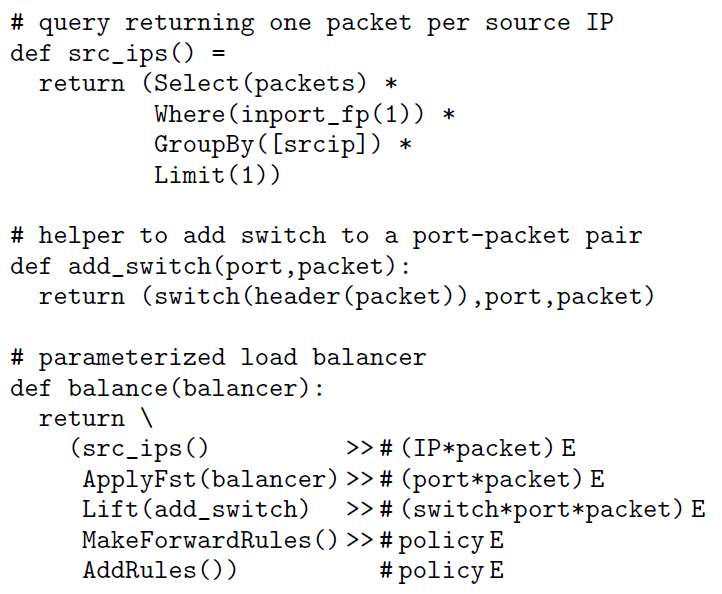
\includegraphics[width=\columnwidth]{images/freneticSimpleLoadBalancer.PNG}
	\caption{Einfacher Load Balancer mit Frenetic \cite{4}[S. 285]}
	\label{fig:freneticSimpleLoadBalancer}
\end{figure}
Die Funktion src\_ips() ermittelt über eine Frenetic Query eine Liste aller Pakete mit unterschiedlicher Quell-IP-Adresse. Ein Paket mit bestimmter IP-Adresse taucht in diesem Set dank Limit(1) nur einmal auf.\\
Die balance-Methode hat den Übergabeparameter balancer, welcher eine Event Function darstellt, die den zugehörigen Port einer IP-Adresse berechnen kann. \cite{4}[S. 286]\\
Folglich wird für jede Quell-IP-Adresse ein Port berechnet, und danach über bekannte Library-Funktionen die passende Regel erzeugt und im Switch gespeichert.

\subsection{Architektur}
Nach der Betrachtung und Analyse der Programmierkonstrukte, möchten wir uns die Architektur von Frenetic ansehen.\\
In Abbildung \ref{fig:freneticArchitecture} sind die 3 Schichten der Frenetic Architektur zu sehen. Wie bereits erwähnt, baut Frenetic auf dem bekannten NOX Controller auf. Dieser arbeitet bereits event-gesteuert und kommuniziert direkt mit dem Frenetic Run-Time System. Dieses wiederum kommuniziert event-gesteuert mit dem Frenetic-Programm, dessen Sprachkonstrukte in den vorherigen Kapiteln beschrieben wurden.\\
\newline
Den Hauptteil der Architektur definiert offensichtlich das Run-Time System, welches die Schnittstelle zwischen dem Low-Level-Interface NOX und dem High-Level Frenetic-Programm ist. \cite{4}[S. 287]\\
Das Run-Time System führt in gewisser Weise Buch über das Installieren und Löschen von Switch-Regeln und verwaltet dazu 3 globale Datenstrukturen: \cite{4}[S. 287]
\begin{itemize}
	\item \textbf{policy}\\
	Ein Wörterbuch, in dem zu jedem Switch der Satz High-Level-Regeln gespeichert wird.
	\item \textbf{flows}\\
	Ein Set, welches alle aktuell installierten Low-Level-Regeln im Netzwerk speichert.
	\item \textbf{subscribers}
	Ein Set aus Tupeln mit je: Definition der Paket-Headers, Event, Byte-/Paket-Zähler, Liste offener Statistik-Anfragen
\end{itemize}
\begin{figure}[h]
	\centering
	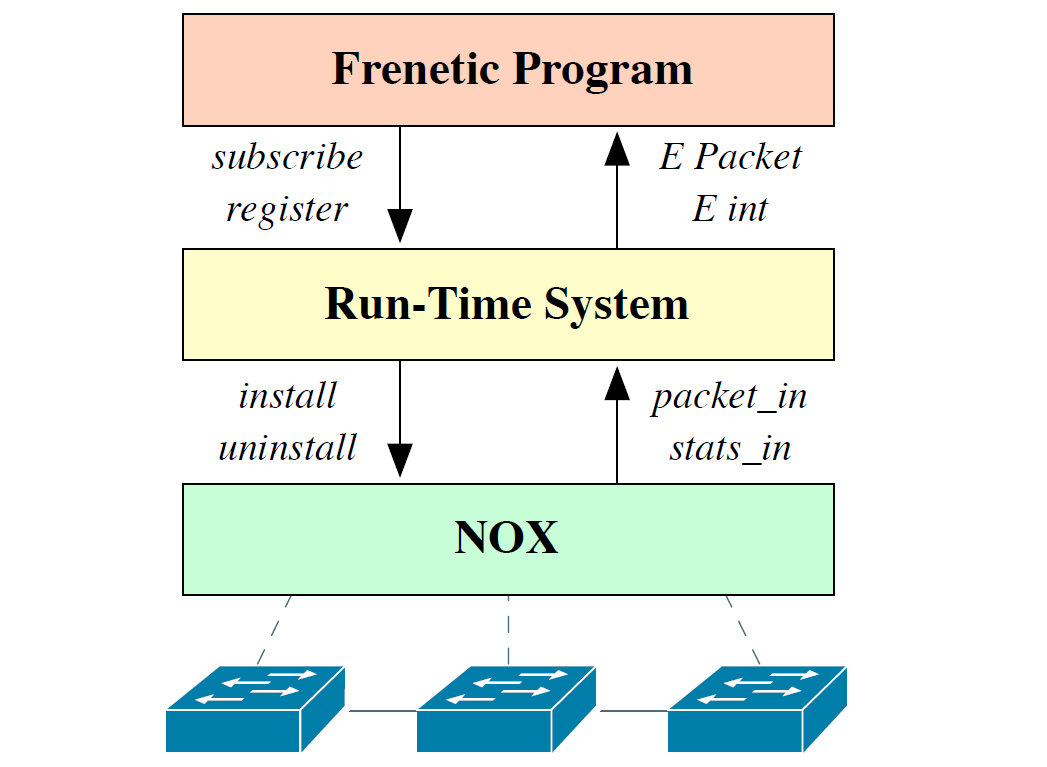
\includegraphics[width=\columnwidth]{images/freneticArchitecture.PNG}
	\caption{Architektur von Frenetic \cite{4}[S. 287], \cite{3}[S.5]}
	\label{fig:freneticArchitecture}
\end{figure}
Zur Umsetzung der High-Level-Regeln in Low-Level-Switch-Regeln reagiert das Run-Time System auf den aktuellen Netzwerkverkehr.\\
Zu Beginn besteht die Annahme, dass alle FlowTables in den Switches leer sind, da noch keine Pakete im Netzwerk unterwegs sind. Folglich werden alle Pakete zuerst einmal über den packet-in-Handler ans Run-Time System weitergeleitet. Dort werden nacheinander folgende Berechnungen durchgeführt \cite{4}[S. 287-288]:
\begin{enumerate}
	\item Suche in \textit{subscribers} alle Einträge, auf die der Paket-Header matched
	\item Verteile das Paket an alle ermittelten Subscribers
	\item Ermittle aus \textit{policy} alle Aktionen, die für diesen Paket-Header durchgeführt werden sollen.
	\item Ausführung
		\subitem Sofern keine Subscribers existieren...\\
		Installiere Switch-Regeln für identische Pakete, damit der Controller in Zukunft nicht unnötig belastet wird.
		\subitem Sofern Subscribers existieren...\\
		Installiere \underline{keine} Switch-Regeln, sondern leite das Paket direkt an den Switch mit den ermittelten Aktionen weiter.
\end{enumerate}
Statistikanfragen werden vom Run-Time System grundsätzlich anders abgearbeitet. Für jeden Subscriber wird eine Warteschleife ausgeführt, bis der Timeout abläuft. Dann wird für alle passenden EInträge aus \textit{flows} die Abfrage nach Byte- und Paket-Zähler der Switches gestartet.\\ 
Sobald die Werte über den stats\_in Handler eintreffen, wird die Anfrage aus den offenen Anfragen des Subscribers entfernt. \cite{4}[S. 288]\\
\newline
Die Library der funktionalen reaktiven Programmierung ist nicht wie üblich mit einer pull-basierten Strategie \cite{13}, sondern über eine push-basierte Strategie \cite{13} umgesetzt. \cite{4}[S. 288]\\
Pull-basierte Strategien arbeiten demand-driven, d.h. das Programm muss aktiv Daten anfordern. Push-basierte Strategien, wie z.B. Frenetic oder GUIs reagieren dagegen auf Datenströme, sobald sie auftreten. \cite{13}[S. 25]

\subsection{Skalierbarkeit und Performance}
Da die Frenetic Architektur auf NOX aufbaut und gleichzeitig ein deutlich höheres Abstraktionslevel erreicht, ist es interessant, mehrere Benchmarks von Frenetic und NOX direkt zu vergleichen.\\
Dabei stellt sich vorrangig die Frage, wie groß der Leistungsverlust durch das hohe Abstraktionslevel wirklich ist und wie gut sich Frenetic im Vergleich zu NOX skalieren lässt.\\
\newline
Der \textit{All-Pais Connectivity} Benchmark aus Abbildung \ref{fig:freneticBenchmarkAllPairsConnectivity} zeigt die Datenmenge an, die je bei NOX und Frenetic über den Controller läuft, wenn alle Hosts im Netzwerk sich gegenseitig Ping-Pakete senden. Dies prüft ob die Kommunikation zwischen allen Netzwerkteilnehmern korrekt funktioniert. \cite{4}[S. 288]\\
Zu sehen ist, dass vor allem bei vielen Hosts, also großen Netzwerken (mehr als 25 Hosts), die Frenetic Architektur den Controller deutlich entlastet.
\begin{figure}[h]
	\centering
	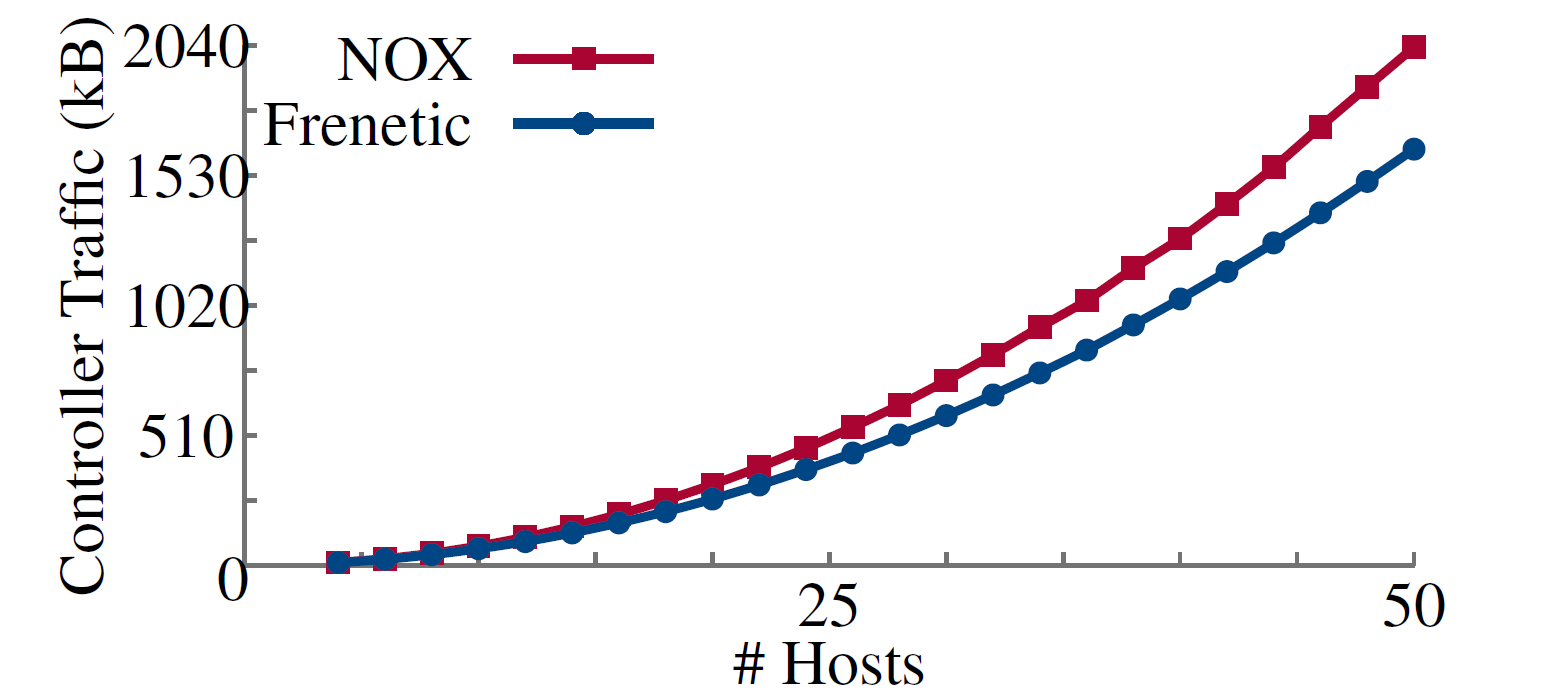
\includegraphics[width=\columnwidth]{images/freneticBenchmarkAllPairsConnectivity.PNG}
	\caption{Frenetic vs. NOX: All Pairs Connectivity Benchmark \cite{4}[S. 289]}
	\label{fig:freneticBenchmarkAllPairsConnectivity}
\end{figure}
\newline
Der \textit{Web Statistics} Benchmark aus Abbildung \ref{fig:freneticBenchmarkWebStatistics} zeigt auch wieder die Datenmenge an, die über den Controller läuft. In diesem Benchmark sendet jeder Host einen einzigen HTTP-Request ab und der Controller misst alle 5 Sekunden den aggregierten HTTP-Netzwerkverkehr. So können die einfachen Monitoring-Kapazitäten ermittelt werden. \cite{4}[S. 288]\\
Bei diesem Benchmark produzierte Frenetic marginal mehr Datenverkehr auf dem Controller, wenn die Anzahl der Hosts nach oben skaliert wurde. Trotzdem muss gesagt werden, dass der Anstieg absolut konstant und nicht etwas sprunghaft wie bei NOX verläuft.
\begin{figure}[h]
	\centering
	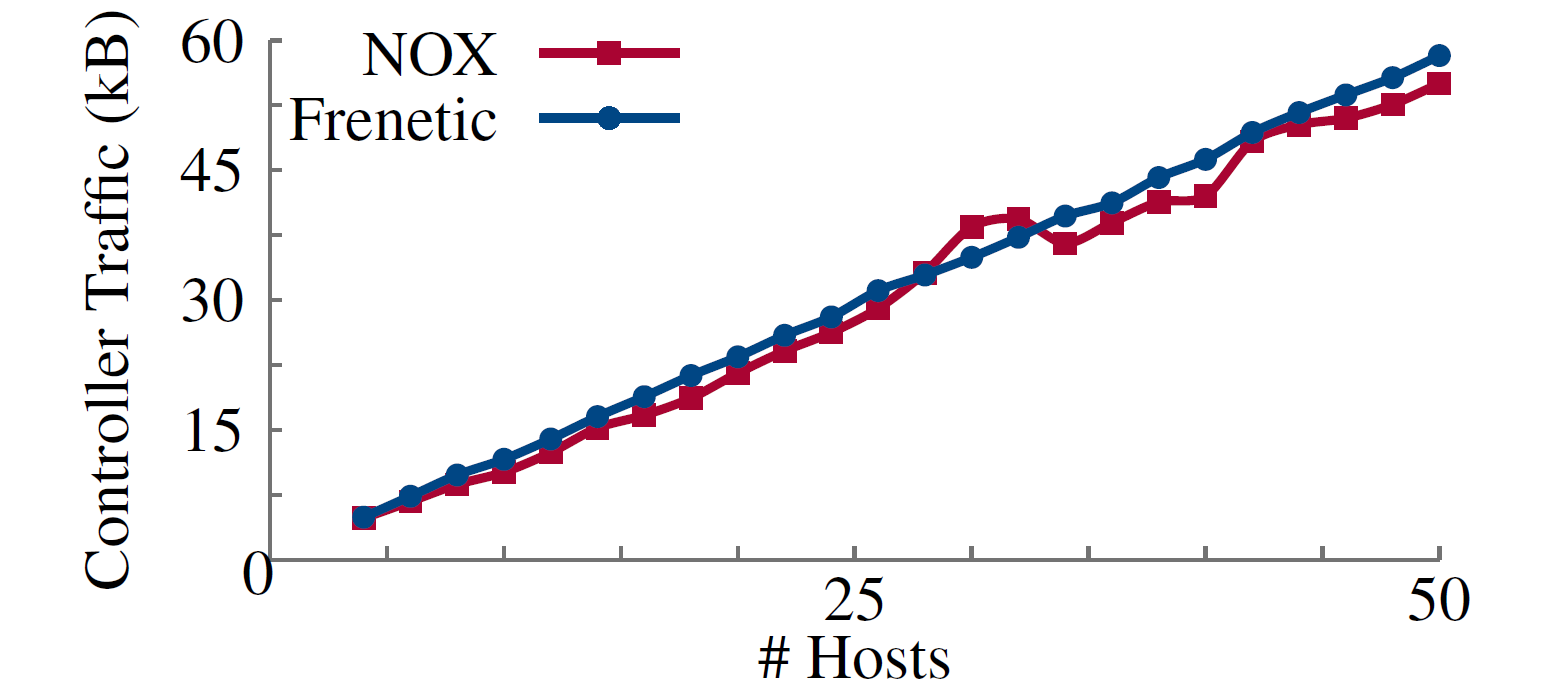
\includegraphics[width=\columnwidth]{images/freneticBenchmarkWebStatistics.PNG}
	\caption{Frenetic vs. NOX: Web Statistics Benchmark \cite{4}[S. 289]}
	\label{fig:freneticBenchmarkWebStatistics}
\end{figure}
\newline
Der Heavy Hitters Benchmark aus Abbildung \ref{fig:freneticBenchmarkHeavyHitters} stellt in gewisser Weise eine Erweiterung des All-Pais Connectivity Benchmarks aus Abbildung \ref{fig:freneticBenchmarkAllPairsConnectivity} dar. Der Unterschied liegt darin, dass je Host zufällig Pings an andere Hosts im Netzwerk gesendet werden. Der Controller berechnet dazu eine Statistik für jeden einzelnen Host und soll die Hosts mit den meisten gesendeten Paketen auflisten. \cite{4}[S. 288]\\
Auch hier ist wieder zu sehen, dass Frenetic weniger Datenverkehr produziert als NOX, wenn es nach oben skaliert wird.
\begin{figure}[h]
	\centering
	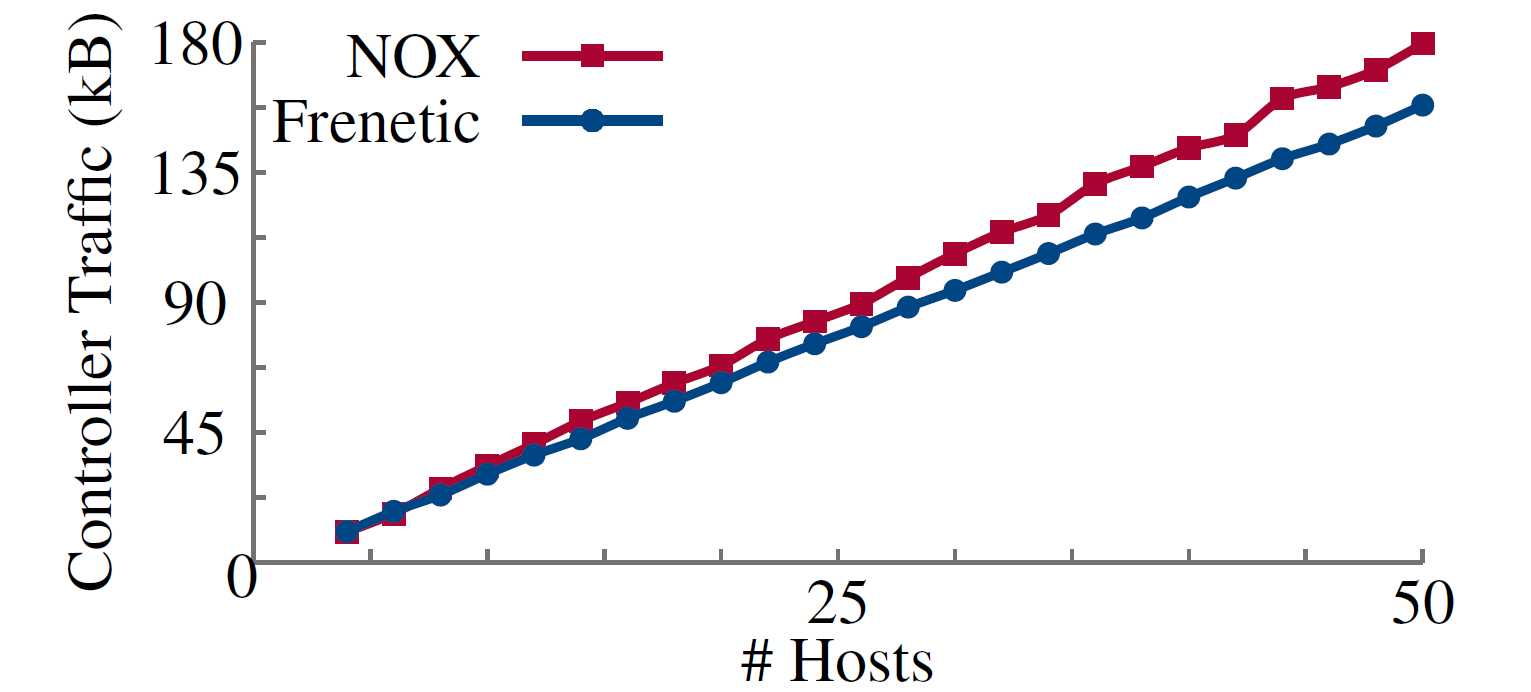
\includegraphics[width=\columnwidth]{images/freneticBenchmarkHeavyHitters.PNG}
	\caption{Frenetic vs. NOX: Heavy Hitters Benchmark \cite{4}[S. 289]}
	\label{fig:freneticBenchmarkHeavyHitters}
\end{figure}
\newline
Zusammenfassend kann gesagt werden, dass Frenetic bezüglich der Skalierbarkeit definitiv im Schnitt besser ist als NOX.\\
Bezüglich der Performance wird behauptet, dass Frenetic-Programme nahezu die gleiche Leistung erreichen als NOX-Programme, jedoch existieren hierzu keine genauen Daten. \cite{4}[289]

\section{Maple}
Eine weitere High-Level Programmiersprache für Software-defined Networks (SDN) ist Maple. Sie basiert auf dem Konzept der Algorithmic Policies, zu deutsch ungefähr algorithmische Strategien.\\
Maple verfolgt anders als Frenetik keinen deklarativen oder funktionalen Ansatz, sondern den klassischen Imperativen Programmieransatz. Daher kann in fast jeder bekannten Sprache wie z.B. Java oder Haskell programmiert werden. \cite{7}[S. 89]

\subsection{Architektur}
In Abbildung \ref{fig:mapleArchitecture} ist die Architektur von Maple, aufgeteilt in das User und das System Level, zu sehen.\\
Ziel ist es, dass der Programmierer nur noch ein einziges Programm f definiert (User Level), welches für alle Pakete abgearbeitet wird. Ein Optimizer und ein Run-Time Scheduler kümmern sich um die Verwaltung der Low-Level-Regeln (System Level). \cite{7}[S. 89]
\begin{figure}[h]
	\centering
	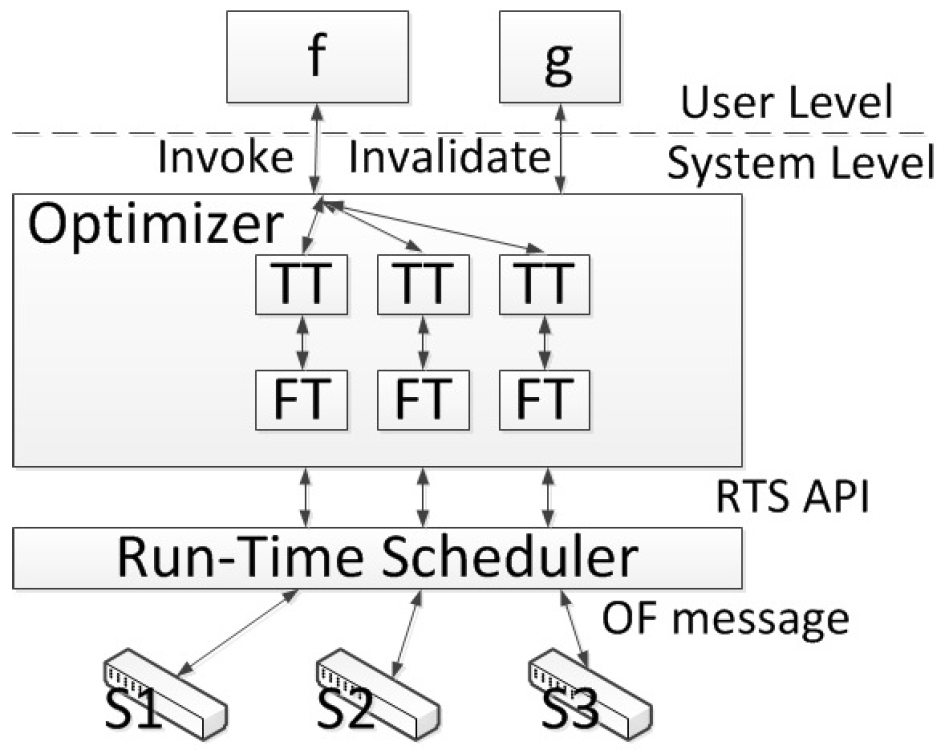
\includegraphics[width=\columnwidth]{images/mapleArchitecture.PNG}
	\caption{Maple Architektur \cite{7}[S. 89] \newline TT = Trace Tree, FT = Flow Table, S.. = Switches}
	\label{fig:mapleArchitecture}
\end{figure}
\newline
Die Anbindung der Switches S1,S2,S3,... erfolgt parallel auf dem Run-Time Scheduler. Ebenso zwischen dem Run-Time Scheduler und dem Optimizer (RTS API).

\subsection{Optimizer}
Der Optimizer stellt die oberste Ebene des Systemlevels dar und gleichzeitig die elementarste. Für jedes Paket erneut das Programm f zu durchlaufen, würde spätestens bei der Skalierung des Netzwerks sehr ineffizient werden. Daher werden sogenannte \textit{Traces} bisheriger Programmdurchläufe in Form von Entscheidungsbäumen gecached, um gleichartige Pakete schnell abarbeiten zu können. \\
Ebenso kann es möglich sein, dass Pakete, die nur die gleiche Ziel-IP-Adresse besitzen, trotzdem den gleichen Weg im Programm nehmen und damit auf die gleiche Weise behandelt werden könnten. \cite{10}[S. 48-49], \cite{7}[S. 89-90]\\
Die sogenannten Trace Trees (TT) (siehe Abbildung \ref{fig:mapleArchitecture}) werden erzeugt und erweitert, sobald die Algorithmic Policy f auf einem bestimmten Paket durchlaufen wurde. \cite{7}[S.90], \cite{10}[S. 48-51]\\
Trace Trees sind folglich immer eine aktuelle Momentaufnahme und repräsentieren nur die bislang durchlaufenen Teile des Programms. Ein Beispiel für solch einen Baum zeigt Abbildung \ref{fig:mapleTraceTree}.\\
Pakete mit TCP-Ziel-Port 22 werden zum aktuellen Zeitpunkt generell gedropped, ebenso diejenigen, mit Ethernet-Ziel-Port 2. Hat ein Paket nicht TCP-ZielPort 22, aber Ethernet-Ziel-Port 4 und kommt gleichzeitig von Ethernet-Port 6, so wird es an Port 30 im Switch weitergeleitet. \cite{7}[S. 93]
\begin{figure}[h]
	\centering
	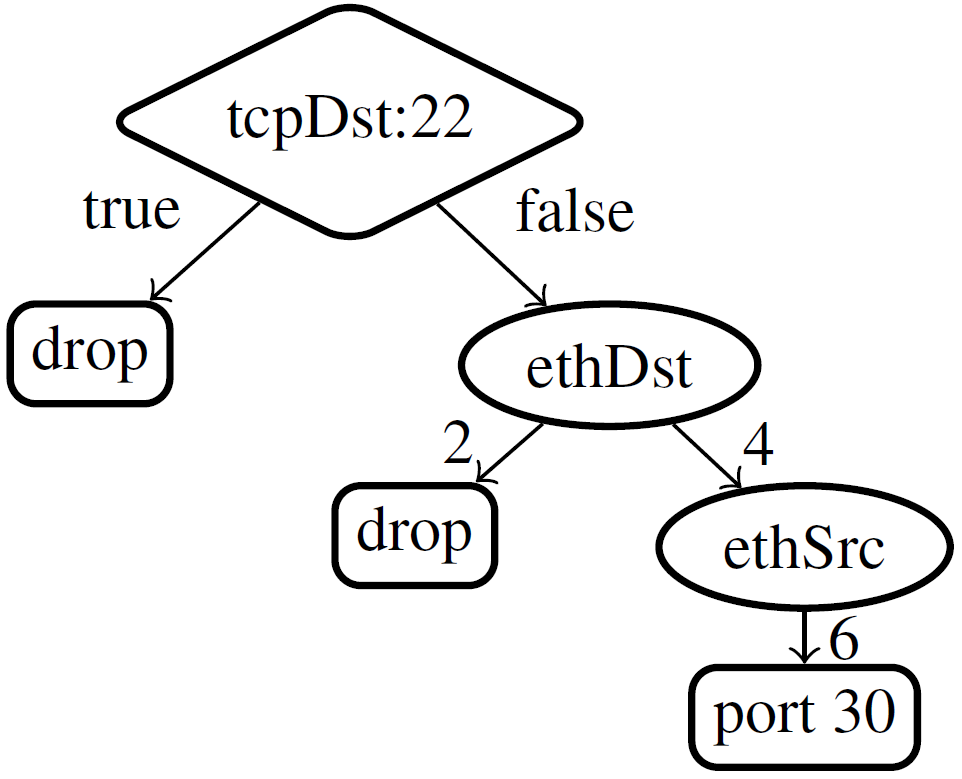
\includegraphics[width=0.5\columnwidth]{images/mapleTraceTree.PNG}
	\caption{Beispiel: Trace Tree in Maple \cite{7}[S. 93]}
	\label{fig:mapleTraceTree}
\end{figure}
\newline
Die Berechnung eines Trace Trees anhand einer Flow Table funktioniert genauso effizient wie die Berechnung einer Flow Table anhand eines Trace Trees. Sobald keine passende Regel in der Flow Table gefunden wird, wird für das entsprechende Paket das Programm im User Level durchlaufen, danach der Trace Tree(s) aktualisiert und daraus wiederum die Flow Table(s) angepasst. \cite{7}[S. 90-92]\\
Maple beinhaltet einige Algorithmen zur Optimierung der erzeugten Trace Trees. So können beispielsweise nicht mehr erreichbare Teilzweige entschlankt oder andere zusammengefasst werden, wenn sie abschnittsweise das gleiche Ergebnis liefern. Daraus folgt, dass auch ständig die Flow Tables automatisch optimiert werden.\\
Aufgrund der benötigten hohen Rechenleistung des Controllers, gerade für hochskalierte Netzwerke, sieht die Architektur explizit Multi-Prozessor-Server vor. \cite{7}[S. 92-95]

\subsection{Skalierbarkeit und Performance}
Gleich wie im Falle von Frenetic interessiert uns auch bei Maple der Vorteil der Technologie. Der Fokus liegt dabei vor allem auf der Skalierbarkeit und der Performance.\\
Die hohe Qualität der Optimierungsalgorithmen für die Flow Table Einträge ist in Abbildung \ref{fig:mapleMissRate} zu sehen.
\begin{figure}[h]
	\centering
	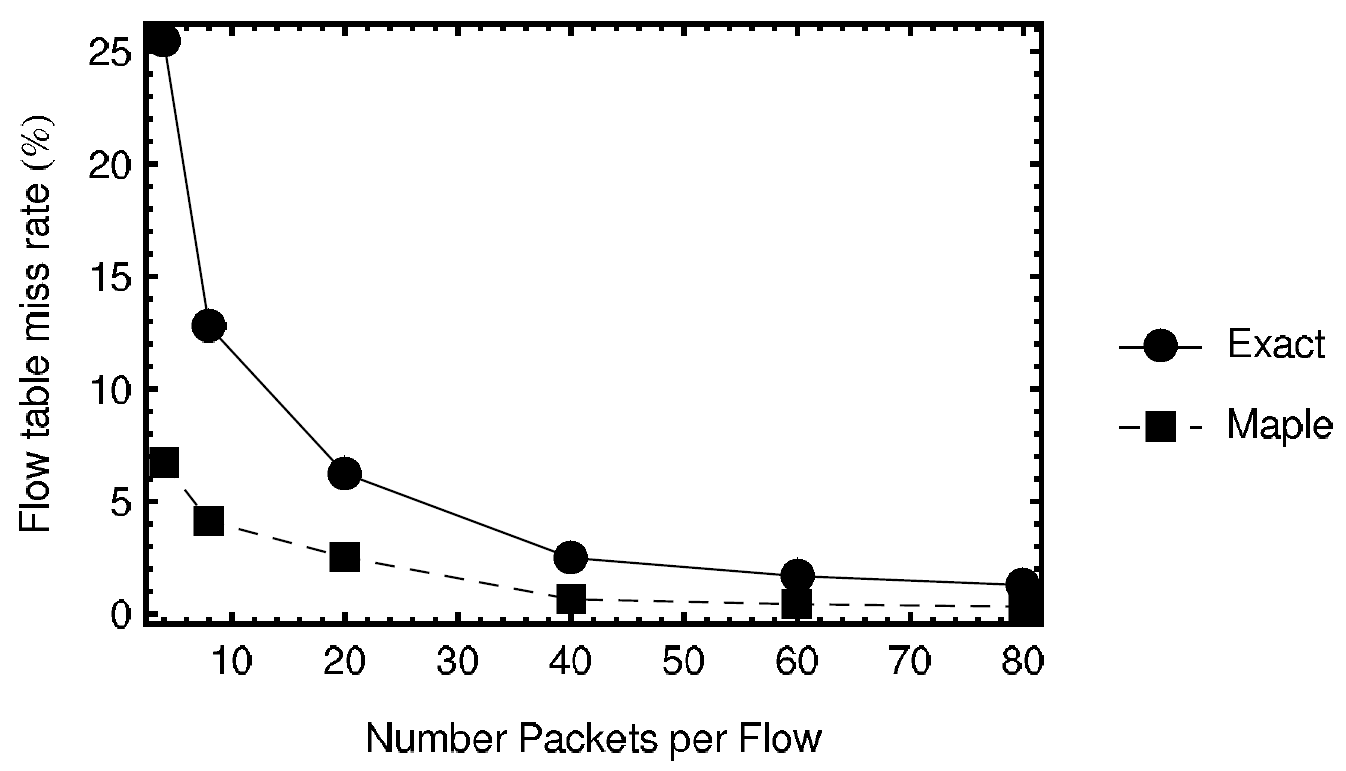
\includegraphics[width=\columnwidth]{images/mapleMissRate.PNG}
	\caption{Benchmark: Flow Table miss rate für Maple \cite{7}[S. 97]}
	\label{fig:mapleMissRate}
\end{figure}
\newline
Auf der y-Achse ist dabei der Prozentsatz an Paketen, welche nicht im Switch weitergeleitet werden können, sondern an den Controller übermittelt werden, aufgezeigt. Maple liegt gegenüber dem Controller, welcher die Pakete exakt auf die Flow Table matched deutlich vorne. Maple erreicht dies durch optimierte Regeln, welche nur noch auf die Quell- und Ziel-IP-Adresse gemappt werden. \cite{7}[S. 96]\\
Ein weiterer Benchmark ist in Abbildung \ref{fig:mapleConnectionTime} dargestellt. Hierfür wurden die Ende-zu-Ende-Zeiten von HTTP-Datenverkehr zwischen den einzelnen Hosts ermittelt. Dadurch kann ein Eindruck der Performance gewonnen werden. \cite{7}[S. 96-97]
\begin{figure}[h]
	\centering
	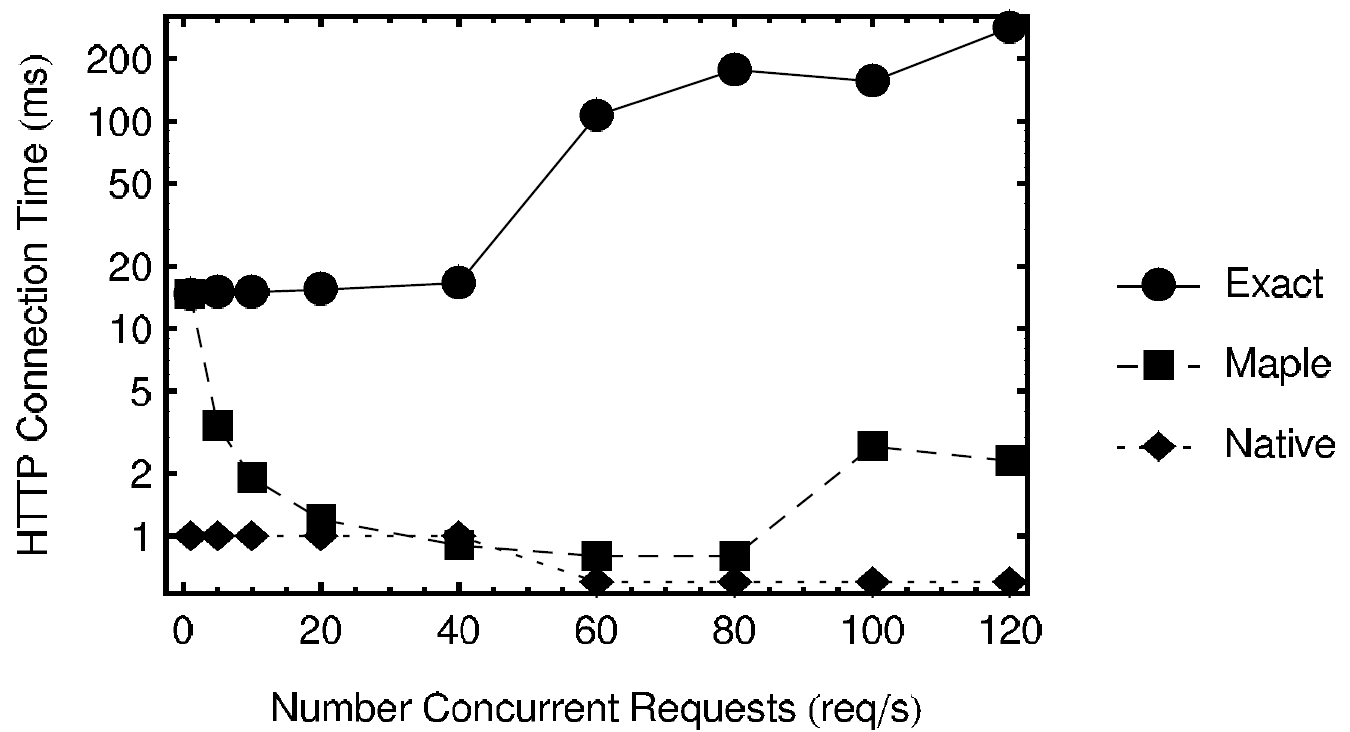
\includegraphics[width=\columnwidth]{images/mapleConnectionTime.PNG}
	\caption{Benchmark: HTTP Connection Time für Maple \cite{7}[S. 97]}
	\label{fig:mapleConnectionTime}
\end{figure}
\newline
Mit steigender Datenrate sinkt die Verbindungszeit für Maple auf rund 1-2 ms, während sie beim exakten Matching ein Vielfaches darüber liegt. Der Anstieg ab etwa 80 Anfragen pro Sekunde wird mit der Auslastung der Switches begründet.\\
Dennoch fällt das Fazit in diesem Fall phänomenal gut für Maple aus. \cite{7}[S. 97]\\
\newline
Am interessantesten ist jedoch der Performance-Vergleich von Maple im Gegensatz zu Frenetic oder NOX.\\
Bezüglich der Skalierbarkeit mit Steigerung der Prozessorkerne kann Maple in Abbildung \ref{fig:mapleDurchsatz} den vollen Trumpf gegenüber NOX ausspielen. Wie im Frenetic-Kapitel bereits gesehen, liegt Frenetic in etwa auf Höhe von NOX bezüglich Durchsatz und Performance.
\begin{figure}[h]
	\centering
	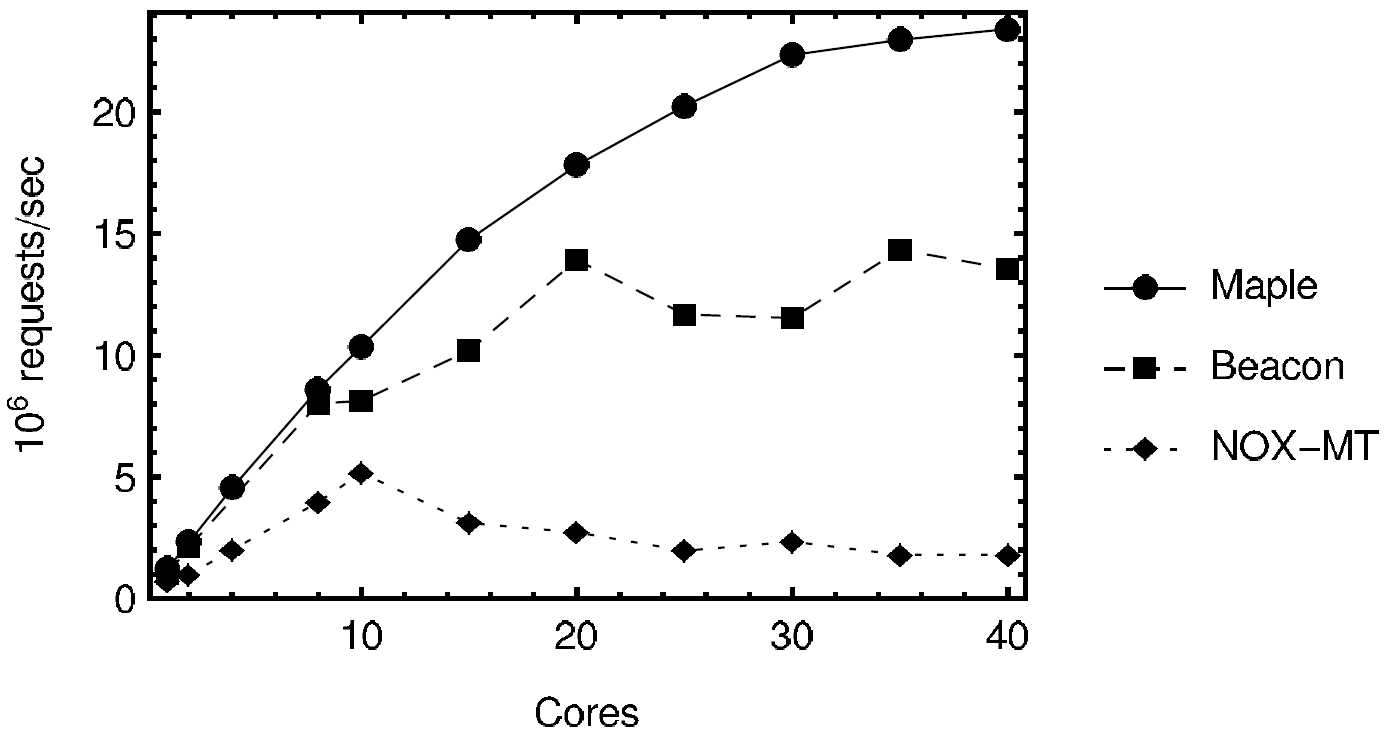
\includegraphics[width=\columnwidth]{images/mapleDurchsatz.PNG}
	\caption{Vergleich des Datendurchsatzes \cite{7}[S. 98]}
	\label{fig:mapleDurchsatz}
\end{figure}
\newline
NOX und damit auch Frenetic skalieren nur minimal oder garnicht durch die Spendierung mehrerer Prozessoren für den Controller. Hier kann Maple einen vielfach höheren Durchsatz durch die strikte Parallelarchitektur erzielen.\\
Dieselbe Beobachtung kann bezüglich der mittleren Antwortzeiten in Abbildung \ref{fig:mapleResponseTime} gemacht werden.
\begin{figure}[h]
	\centering
	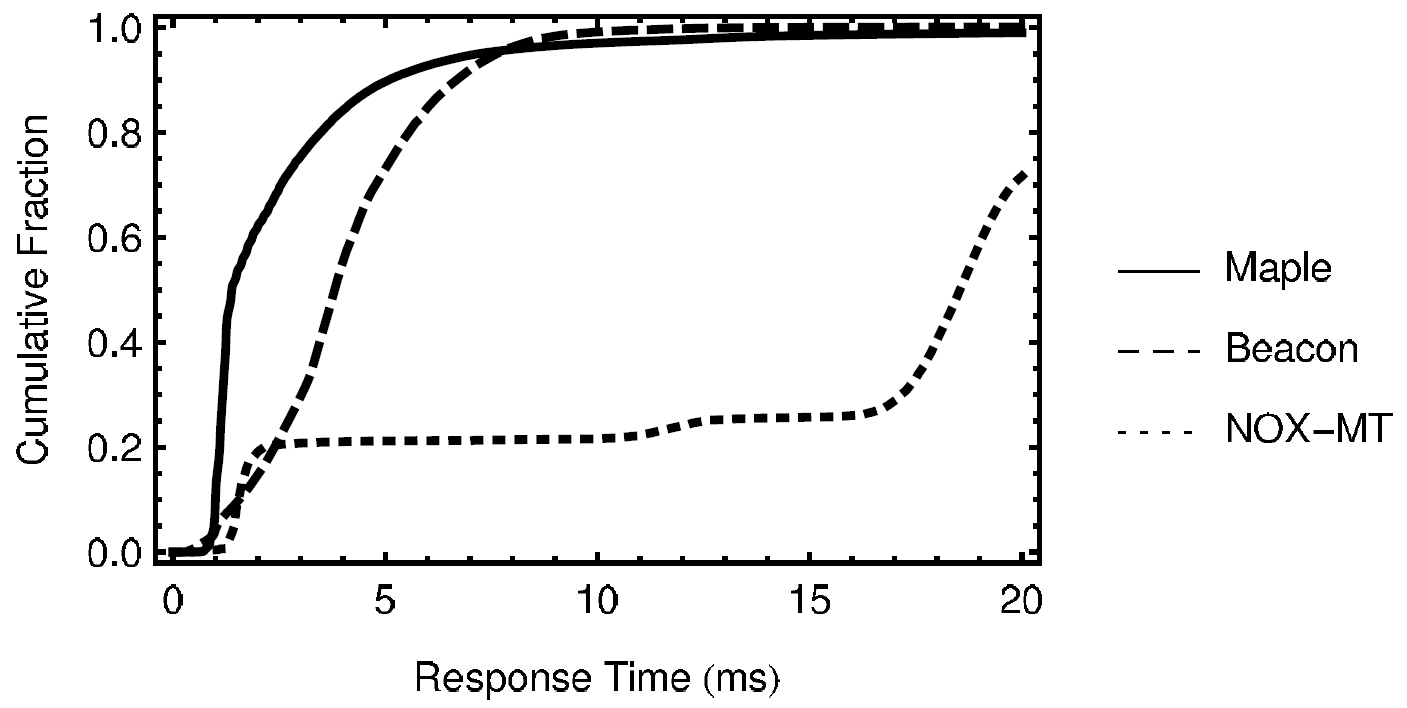
\includegraphics[width=\columnwidth]{images/mapleResponseTime.PNG}
	\caption{Vergleich der mittleren Antwortzeiten \cite{7}[S. 98]}
	\label{fig:mapleResponseTime}
\end{figure}
\newline
Währen Maple im Median bei etwa 1 ms liegt, benötigt NOX und damit auch Frenetic im Median schon etwa 17 ms. Damit ist Maple in diesem Benchmark etwa um den Faktor 17 schneller also NOX oder Frenetic. \cite{7}[S. 98]

\section{Fazit und Zusammenfassung}
Zusammenfassend kann gesagt werden, dass Frenetic und Maple auf ganz unterschiedlichen Architekturen und Philosophien basieren.\\
Während Frenetic auf dem älteren NOX Controller aufbaut und eine Abstraktionsebene für diesen mittels funktionaler Programmierung darstellt, verfolgt Maple den iterativen Ansatz. Maple hat gefühlt das noch höhere Abstraktionslevel, da Regeln aus dem Programmdurchlauf eines iterativen Programms erzeugt werden. Dazu kommt nocht die Parallelarchitektur, welche sich extrem gut skalieren lässt.\\
Positiv zu nennen ist aber auch, dass Frenetic in etwa gleiche Benchmarkwerte erzielt wie der darunter liegende NOX-Controller. Somit schluckt die Abstraktionsebene für den Benutzer nahezu kaum Systemleistung. Trotzdem fällt es vermutlich vielen iterativen Programmierern schwer, gedanklich dem funktionalen Ansatz zu folgen, der prinzipiell gegen die klassische Softwareentwicklung strebt.\\
Sobald als Controller ein potenter Server mit vielen Prozessoren zur Verfügung steht und das Netzwerk schnell ziemlich groß wird, für kein Weg mehr an Maple vorbei. Bei Multiprozessorsystemen hat Frenetic oder NOX bezüglich Performance und Skalierbarkeit kaum noch eine Chance. Dazu kommt noch die vermeintliche Hürde der funktionalen Programmierung, was diese Techniken im Allgemeinen uninteressant machen dürfte.
% Abbildungsverzeichnis
\listoffigures
% Literaturverzeichnis (quellen.bib)
\bibliography{quellen}{}
\bibliographystyle{plain}

\end{document}